%%%% This CV has been greatly influence by
%%%% the extended fancy cv from Carmine Benedetto.
%%%% I thank him for the excellent work. Unfortunately 
%%%% it wouldn't compile on my machine. So I worked it out myself.

\documentclass{scrartcl} 
\usepackage[ngerman]{babel}% deutsche Trennregeln
\usepackage{microtype}% verbesserter Randausgleich
\usepackage[utf8]{inputenc}
\usepackage{graphicx}
\usepackage{color}
\usepackage{xcolor}
\usepackage[obeyspaces]{url} 
\usepackage[left=0.5cm,top=0cm,right=1.5cm,bottom=2.5cm,nohead,nofoot]{geometry}

\makeatletter
\setlength{\@fptop}{40pt}
\makeatother

\usepackage{pdfcomment}
% Fix incorrect display of tooltips (http://tex.stackexchange.com/a/74340/3323)
\makeatletter
\renewcommand{\pc@annot@tooltip}%
{%
  /TU (\pc@pdfenc@contents)\space%
  /T (tooltip \thezref@unique)\space%
  /C [0 0 0]\space%
  /FT/Btn\space%
  /Ff 65536\space%
  /H/N\space%
}%


\newcommand{\entry}[4]{%
  \parbox[t]{3cm}{#1}&\parbox[t]{10cm}{%
    \textbf{#2}%
    \hfill%
    {\footnotesize \color{pblue} #3}\\%
    #4\\ \vspace{\parsep}%
  }\\}
  
\newcommand{\entryy}[4]{%
  \parbox[t]{2cm}{#1}&\parbox[t]{12cm}{%
    \textbf{#2}%
    \hfill%
    {\footnotesize \color{pblue} #3}\\%
    #4\\ \vspace{\parsep}%
  }\\}  
  
\definecolor{white}{RGB}{255,255,255}

\definecolor{darkgray}{HTML}{333333}
\definecolor{gray}{HTML}{4D4D4D}
\definecolor{lightgray}{HTML}{999999}

\definecolor{green}{HTML}{C2E15F}
\definecolor{orange}{HTML}{FDA333}
\definecolor{purple}{HTML}{D3A4F9}
\definecolor{red}{HTML}{FB4485}
\definecolor{blue}{HTML}{6CE0F1}
\definecolor{pblue}{HTML}{0395DE}


\usepackage{hyperref}
\hypersetup{
    pdftitle={},
    pdfauthor={},
    pdfsubject={},
    pdfkeywords={},
    colorlinks=false,       % no lik border color
   allbordercolors=white    % white border color for all
}
 
\pagestyle{empty}

\begin{document}
\begin{figure}[htb]
\begin{minipage}[t]{0.25\textwidth}
	\flushright
	\section*{\hfill \color{pblue} Address}
	\vspace{-4mm}
	Großbeerenstraße 33\\
	14482 Potsdam\\
	Deutschland\\
	~
	\section*{\hfill \color{pblue} Tel \& Skype}
	\vspace{-4mm}
	$+49~174~6507598$\\
	$+49~331~58256842$\\
	silvio.schwarz\\
	~
	\section*{\hfill \color{pblue} Mail}
	\vspace{-4mm}
	\href{mailto:silvio\_ schwarz@web.de}{silvio{\_}schwarz@web.de}\\
	\href{mailto:silvioschwa@gmail.com}{silvioschwa@gmail.com}
	~
	\section*{\hfill \color{pblue} Web}
	\vspace{-4mm}
%	\small
	\href{https://www.github.com/silvioschwarz}{github.com/silvioschwarz} \\
	\href{https://www.linkedin.com/in/silvioschwarz}{linkedin.com/in/silvioschwarz} \\
	\href{http://www.mathematica-silvio.blogspot.de/}{mathematica-silvio.blogspot}\\
	\href{https://www.silvioschwarz.no-ip.org}{silvioschwarz.no-ip.org}\\(offline -- contact me!)\\
~
	\section*{\hfill \color{pblue} OS Preferences}
	\vspace{-2mm}
	\textbf{GNU/Linux}
\includegraphics[scale=0.40]{img/5stars.png}
	\textbf{Windows}
\includegraphics[scale=0.40]{img/4stars.png}
    \textbf{MacOS}
\includegraphics[scale=0.40]{img/1stars.png}\\
~
    \section*{\hfill \color{pblue} Programming}
	\vspace{-2mm}
	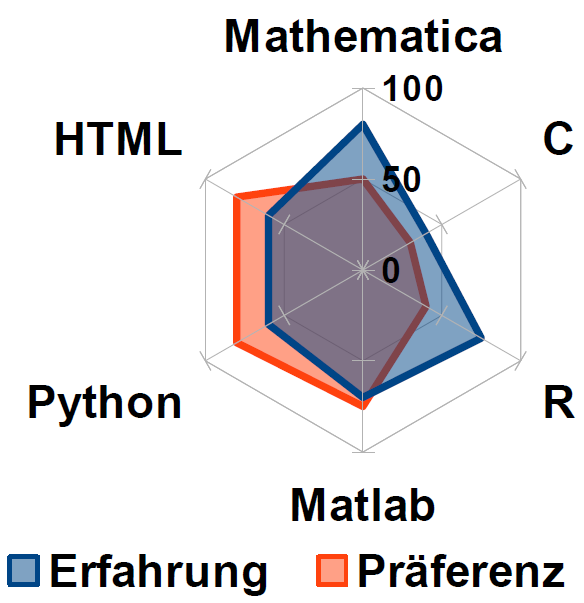
\includegraphics[scale=0.65]{img/Programming.png}
	~
	\section*{\hfill \color{pblue} Languages}
	\vspace{-2mm}
	\textbf{German}
\includegraphics[scale=0.40]{img/5stars.png}
	\textbf{English}
\includegraphics[scale=0.40]{img/4stars.png}
    \textbf{Italian}
\includegraphics[scale=0.67]{img/3stars.png}
    \textbf{French}
\includegraphics[scale=0.40]{img/2stars.png}
	\end{minipage}
	\hfill
%	
	\begin{minipage}[t]{0.72\textwidth} 
	{\fontsize{30pt}{62pt}\color{gray} \selectfont {Silvio}{\textbf{Schwarz}}}\\
    {\fontsize{14pt}{24pt}\color{pblue} \selectfont Geophysicist \color{lightgray} (B.Sc.)}\\
	\hrule
	
	    
	\section*{\fontsize{18pt}{24pt}\selectfont Education}
	 \begin{tabular*}{\textwidth}{@{\extracolsep{\fill}}ll}
	    \entry
	    {10/2011 - Present}
	    {Master of Science}
	    {\href{https://www.uni-potsdam.de/}{Universität Potsdam, Germany}}
	    {Earth Science\\
	    Specialization in Geophysics\\
	    Main subjects: Seismology, Probability Theory, Machine Learning, Data Processing\\
	    Thesis: Forecasting Macroseismic Intensities: A Sensitivity Study of a Bayesian Approach}
	    
	    \entry
	    {10/2008 - 09/2011}
	    {\href{https://www.dropbox.com/s/297g1chiby8mrd3/Bachelor-Certificate.pdf?dl=0}{Bachelor of Science}}
	    {\href{https://www.uni-potsdam.de/}{Universität Potsdam, Germany}}
	    {Earth Science\\
	    Main subjects: Physics, Mathematics, Chemistry, Geology\\
	    Thesis: \href{https://www.dropbox.com/s/3kngo4hpb0c47ww/Bachelorarbeit.pdf?dl=0}{\pdftooltip{Simulation von Bodenbewegungsszenarien von Starkbeben (German)}{engl.: Simulating Ground Motion Scenarios of strong Earthquakes}}\\
	    Thesis activity was carried out during a position as student research assistant at University Potsdam.}
	    
	    \entry
	    {08/2000 - 05/2008}
	    {\href{https://www.dropbox.com/s/nsgmvy7o64xb9si/Abiturzeugnis.pdf?dl=0}{Abitur}}
	    {\href{http://www.klosterschule.de/}{Klosterschule Roßleben, Germany}}
	    {Secondary School\\
	    Main subjects: Geography, Mathematics\\
	    Thesis: \pdftooltip{Naturkatastrophen und ihr Einfluss auf das Leben in der Gegenwart (German)}{engl.: Natural Disasters and their Impact on Life in the Present}}
	     \end{tabular*}
	     \vspace{-10mm}
	\section*{\fontsize{18pt}{24pt}\selectfont Experience}
	    \begin{tabular*}{\textwidth}{@{\extracolsep{\fill}}ll}
	    \entry
	    {08/2014 - Present\\ (1 Year 1 Month)}
	    {Student Employee}
	    {\href{https://assecor.de/}{Assecor GmbH, Berlin, Germany}}
	    {Support in documentation of the power supply system of Berlin, Germany for Vattenfall Europe Sales GmbH}
	    
	    \entry
	    {11/2013 - 03/2014 \\ (5 Months)}
	    {Student Employee}
	    {\href{https://assecor.de/}{Assecor GmbH, Berlin, Germany}}
	    {Migration of IT Infrastructure to Windows 7 for\\
	     BIOTRONIK SE \& Co. KG}
	    
	    \entry
	    {09/2012 - 11/2012 \\ (3 Months)}
	    {Internship}
	    {\href{https:///www.wolframalpha.com/}{Wolfram$\mid$Alpha, LLC, Champaigne, IL, USA}}
	    {Research and Development\\
	    Development of geophysical content for Wolfram$\mid$Alpha}
	    
	    \entry
	    {06/2011 - 08/2012 \\ (1 Year 3 Months)}
	    {Student Research Assistant}
	    {\href{https://www.uni-potsdam.de/}{Universität Potsdam, Germany}}
	    {Geophysical prospection, seismological model building, consulting for the Council for Geoscience, Pretoria, South Africa}
	    
	    \entry
	    {02/2011 - 03/2011 \\ (1 Month)}
	    {Internship} 
	    {\href{https://www.zv.uni-leipzig.de/}{Universität Leipzig, Germany}}
	    {Maintenance of the Saxonian Seismological Network, e.g. configuring ISDN routers, collecting data from seismological stations, data preparation for relocation using double difference times}
	    
	    \entry
	    {03/2010 - 05/2010 \\ (3 Months)}
	    {Student Research Assistant}
	    {\href{https://www.uni-potsdam.de/}{Universität Potsdam, Germany}}
	    {Testing Mathematica routines used for seismic hazard assesment}
	    
	    \end{tabular*}
	\end{minipage}
\end{figure}

\begin{figure}[htb]
\begin{minipage}[t]{0.26\textwidth}
\flushright
\section*{\hfill \color{pblue} Places Lived}
	\vspace{-2mm}
	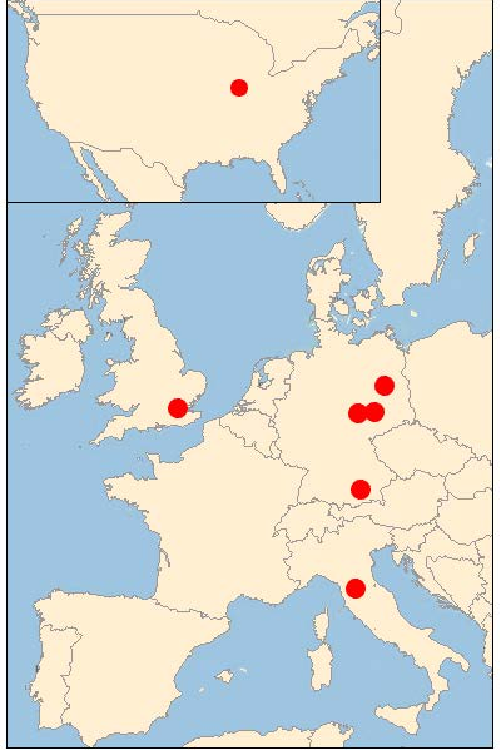
\includegraphics[scale=0.6]{maps.pdf}
\end{minipage}
\hfill
\begin{minipage}[t]{0.72\textwidth} 
	\section*{\fontsize{18pt}{24pt}\selectfont Certificates}
	 \begin{tabular*}{\textwidth}{@{\extracolsep{\fill}}ll}
	    
	    \entryy
	    {12/2014}
	    {\href{https://www.dropbox.com/s/h5ytn8e9sbc4fb6/Coursera-ml-2015.pdf?dl=0}{Machine Learning}}
	    {\href{https://www.coursera.org/}{Coursera, Online Learning}}
	    {Linear Regression, Logistic Regression, Neural Networks, Support Vector Machines, K-Means Clustering, Principal Component Analysis, Cross-Validation}
	    
	    \entryy
	    {12/2014}
	    {\href{https://www.dropbox.com/s/tn8kxs0z9etmw7h/Coursera-Python-2015.pdf?dl=0}{Programming for Everybody (Python)}}
	    {\href{https://www.coursera.org/}{Coursera, Online Learning}}
	    {Basic Introduction to Python}
	     
	     \entryy
	    {08/2012}
	    {\href{https://www.dropbox.com/s/t2jo7ly7o7pwsw0/Italian-B2.pdf?dl=0}{Italian (B2)}} 
	    {\href{http://www.europass.it/de/}{Europass School, Florence, Italy}}
	    {}
	    
	    \entryy
	    {07/2012}
	    {\href{https://www.dropbox.com/s/5zbjm6bgriardhm/Italian-Unicert-I.pdf?dl=0}{Italian (Unicert I)}}
	    {Universität Potsdam}
	    {}
	 \end{tabular*}

	\vspace{2cm}
\begin{flushleft}
\emph{\today}
\end{flushleft}
\begin{flushright}
\emph{Silvio Schwarz}
\end{flushright}
\end{minipage}
\end{figure}
\end{document}